%%%%%%%%%%%%%%%%%%%%%%%%%%%%%%%%%%%%%%%%%%%%%%%%%%%%%%%%%%%%%%%%%%%%%%%%%%%

\documentclass{standalone}

\usepackage{mathptmx}
\usepackage{tikz}
\usetikzlibrary{external}
\tikzexternalize{law-sines}

%% We default to Times.
\renewcommand{\rmdefault}{ptm}
\renewcommand{\ttdefault}{pcr}
%% Enable Times/Palatino main text font.
\normalfont\selectfont

%% A generic triangle.

\begin{document}

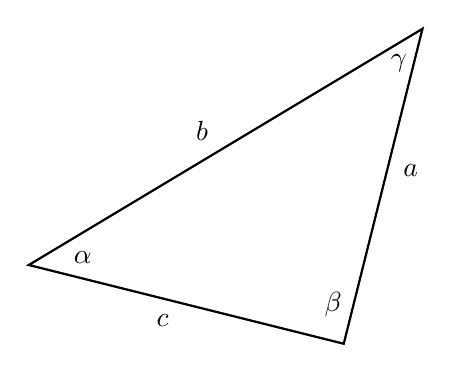
\begin{tikzpicture}[%%
  triangleStyle/.style={-,thick,draw}
]
%%
%%
\coordinate (A) at (0,0);
\coordinate (B) at (4,-1);
\coordinate (C) at (5,3);
%%
%% A generic triangle.
\path[triangleStyle] (A) -- (B) -- (C) -- cycle;
%% Label the angles.
\node at (0.45,0.1) [right] {$\alpha$};
\node at (4.1,-0.5) [left] {$\beta$};
\node at (4.7,2.8) [below] {$\gamma$};
%% Label the sides.
\node at (4.85,1.2) {$a$};
\node at (2.2,1.7) {$b$};
\node at (1.7,-0.7) {$c$};
\end{tikzpicture}

\end{document}
